% ----------------------------------------------------------------------

\section{Appendix - Index in HTML}


\begin{figure}
\lcTex{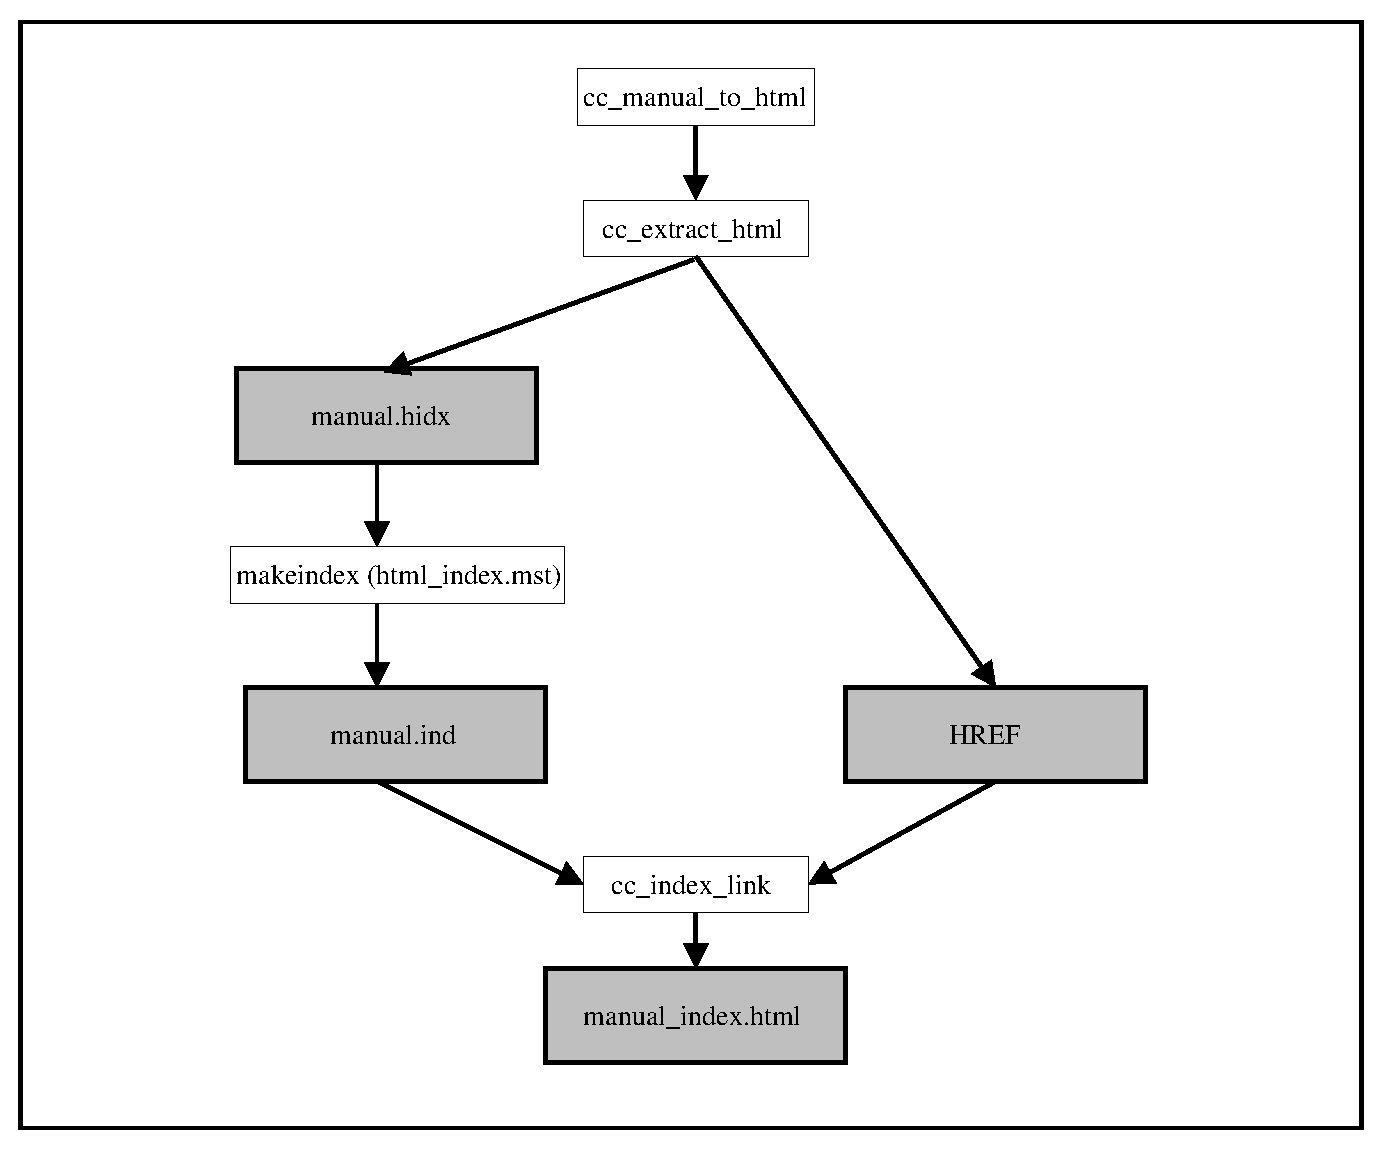
\includegraphics[width=1.0\textwidth]{Manual_tools/tools_index}%
    \caption{The files and tools involved in the 
      process of creating the HTML index.}}
%    \label{ToolsOverviewFig}\figuretopindent
\begin{ccHtmlOnly}
<CENTER>
  <IMG SRC="./tools_index.gif" ALT="Files and tools used in manual writing">
</CENTER>
\end{ccHtmlOnly}
\end{figure}



\normalsize Program \verb|cc_extract_html| produces files
\verb|manual.hidx| and HREF. When the program finds a function that
produces the index position, it creates a new command for the {\tt
  makeindex} program. This new command contains the new index position
and its number. The number differs from the previous one by 2, since
otherwise if these numbers were consecutive it possible that {\tt
  makeindex} would create the page range out of these numbers instead
of separate page numbers.

Also, the program adds to file HREF an address of a link to an
appropriate place with yhe same number as the index position in file
\verb|mannual.hidx|.  After the whole index has been sorted by {\tt
  makeindex} (using the style file \verb|html_index.mst|), a file
\verb|manual.ind| is output. In this file the numbers of the links
have to be combined (attached) with appropriate link from file HREF.
This is done using program \verb|cc_index_link|. If the programm
\verb|cc_manual_to_html| is used with option {\tt -extended}, then the
program combines several \verb|manual.ind| files in to one
\verb|manual.ind| file, and their corresponding \verb|HREF| files into
one \verb|HREF| file. While doing so File \verb|HREF_counter| contains
the information on what should be the next number used for numbering
the links.

Examples:

Index position in file \verb|manual.hidx|:
  \begin{verbatim}
  \indexentry{functionality@ ??? functionality}{1040}
  \end{verbatim}

Link to this position in file \verb|HREF| :
  \begin{verbatim}
  1040 HREF="main.html#Index_anchor_302"
  \end{verbatim}

Sorted position in file \verb|manual.ind|:
 \begin{verbatim}
 <TABLE  CELLPADDING=0 CELLSPACING=0> <TR><TD>  ??? functionality ??? 
   1040 </TD></TR> </TABLE>
 \end{verbatim}

Index position after program \verb|cc_index_link| is run:
 \begin{verbatim}
 <TABLE  CELLPADDING=0 CELLSPACING=0> <TR><TD> 
   <A HREF="main.html#Index_anchor_302">  functionality</A> </TD></TR> </TABLE>
 \end{verbatim}


If a position in the index has many links, the arrows lead to these links.


